% Start writing your answer from here, if you want to use new packages/change something do it in main.tex
\begin{que}
	Download the image of Monalisa from
	\href{https://en.wikipedia.org/wiki/File:Mona_Lisa.jpg}{here}. Read the
	image using matplotlib
	(\href{https://people.ciirc.cvut.cz/~xmatousm/mfftdv/lab1.html}{example}).
	Write a piece of python code to shift the image along the $X$ direction
	by $tx$ pixels where $tx$ is an integer ranging from $-10$ to $+10$
	(so, in total you need to do this for $20$ values). While doing so,
	assign a value of $0$ to unoccupied pixels. For each shift, compute the
	correlation coefficient between the original image and its shifted
	version. Make a plot of correlation coefficients across the shift
	values. Also, generate a normalized histogram for the original image.
	You might need to refer to section 3.3 from this
	\href{https://dl.icdst.org/pdfs/files4/01c56e081202b62bd7d3b4f8545775fb.pdf}{book}.
	You are not allowed to use any inbuilt function for generating the
	histogram. If you are using any other libraries, then please mention
	about them in the pdf.

	\hspace*{\fill} [8 marks]
\end{que}

\begin{tcolorbox}[breakable]
	\begin{sol}
		The image of Mona Lisa was read using the \texttt{matplotlib}
		library. The image was then shifted horizontally by \texttt{tx}
		pixels for each value of \texttt{tx} in the range of -10 to
		+10. The shifting operation was implemented manually, ensuring
		that unoccupied pixels were assigned a value of 0. 

		A custom function \texttt{shiftimg} was created to handle the shifting process:
		\begin{itemize}
			\item If \texttt{tx > 0}, pixels were shifted
			      rightwards by \texttt{tx} units.
			\item If \texttt{tx < 0}, pixels were shifted leftwards
			      by \texttt{tx} units.
			\item If \texttt{tx = 0}, the function returned the
			      original image.
		\end{itemize}
		All the shifted images are displayed in the Jupyter notebook(q8.ipynb). Some of them are displayed below.
		\begin{figure}[H]
			\centering
			\begin{minipage}{0.345\textwidth}
				\centering
				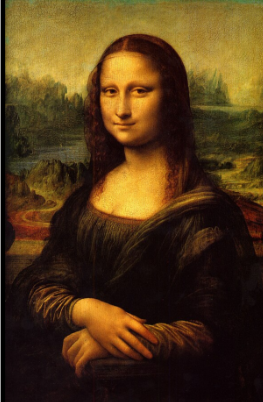
\includegraphics[width=\textwidth]{rightShift10.png}
				\caption{Image with \texttt{tx}=10}
				\label{fig:rightShift}
			\end{minipage}
			\begin{minipage}{0.35\textwidth}
				\centering
				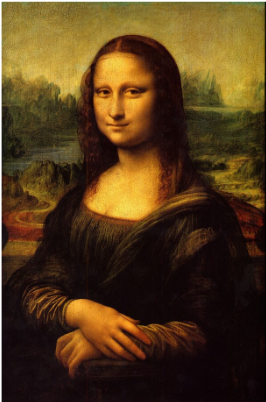
\includegraphics[width=\textwidth]{leftShift5.png}
				\caption{Image with \texttt{tx}=-5}
				\label{fig:leftShift}
			\end{minipage}
		\end{figure}
		

		For each shifted image, the correlation coefficient between the
		original and shifted image was calculated. This coefficient
		quantifies the linear relationship between the two images, with
		values ranging from -1 to 1, where 1 indicates a perfect
		positive correlation, -1 indicates a perfect negative
		correlation, and 0 indicates no correlation. This done using a function \texttt{corrcoef} in \texttt{numpy} library. This function require 2 1-D arrays to determine the correlation coeffiecient. The flattenning of arrays was done using \texttt{.flatten()}.
		Then correlation for each shift is plotted on a graph shown below.  

		\begin{figure}[H]
			\centering
			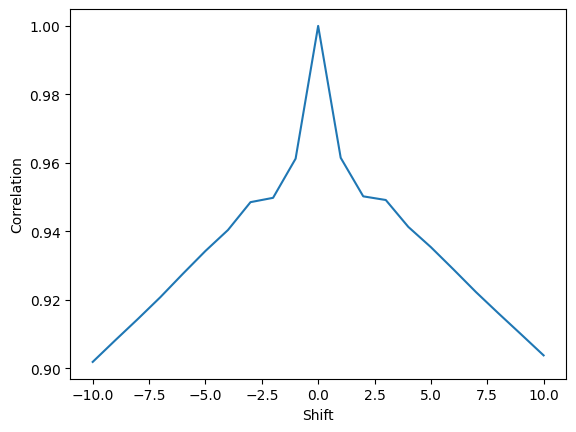
\includegraphics[width=0.8\textwidth]{correlation_plot.png}
			\caption{Correlation Coefficient vs Shift Values}
			\label{fig:corr_plot}
		\end{figure}


		As observed in Figure \ref{fig:corr_plot}, the correlation
		decreases as the shift increases in either direction. This is
		expected as the more the image is shifted, the less it
		resembles the original, resulting in lower correlation values.

		Following this, normalized histogram is plotted for each channel(R,G,B). This is done without use of any library, by creating a function \texttt{draw\_hist} which takes the image of a single channel, transverses through each pixel taking the note of its value and finally each value is divided by the total number of pixels(width*height) to normalize the histogram.

		\begin{figure}[H]
			\centering
			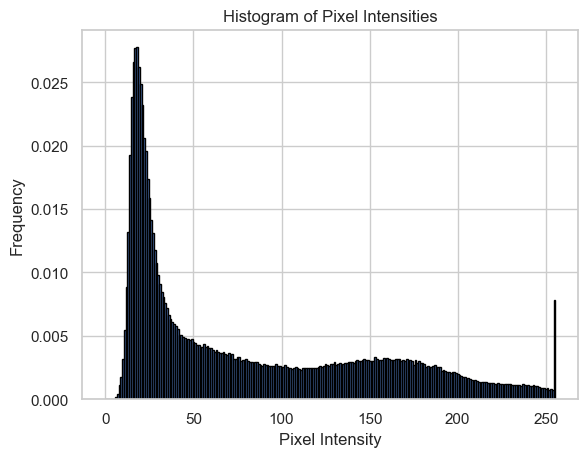
\includegraphics[width=0.8\textwidth]{red_intensity_hist.png}
			\caption{Normalized Histogram of red channel of the Original Image}
			\label{fig:hist_red_plot}
		\end{figure}
		\begin{figure}[H]
			\centering
			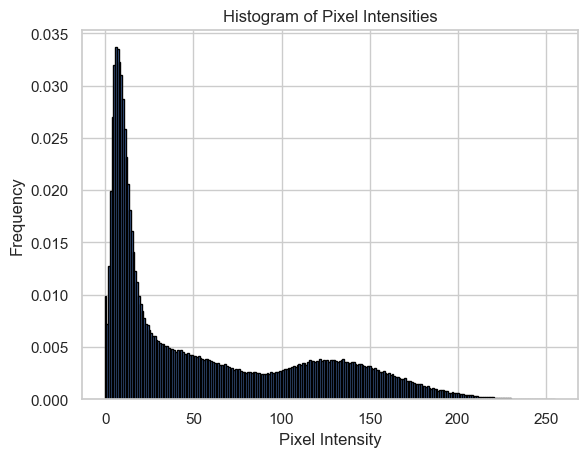
\includegraphics[width=0.8\textwidth]{green_intensity_hist.png}
			\caption{Normalized Histogram of green channel of the Original Image}
			\label{fig:hist_green_plot}
		\end{figure}
		\begin{figure}[H]
			\centering
			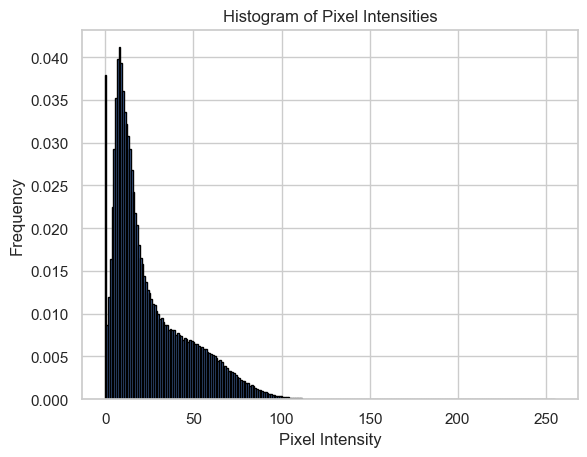
\includegraphics[width=0.8\textwidth]{blue_intensity_hist.png}
			\caption{Normalized Histogram of blue channel of the Original Image}
			\label{fig:hist_blue_plot}
		\end{figure}

		

		
	\end{sol}
\end{tcolorbox}
